\documentclass{entcs} 
\usepackage{prentcsmacro}
\usepackage{graphicx}
\usepackage{xspace}

%
% For semantic.sty
%
\renewcommand{\predicate}[1]{$#1$}% Set predicates in math mode
\setpremisesend{1ex}
\setpremisesspace{1ex}
\setnamespace{0.5ex}

%
% Listings
%
\lstdefinelanguage{Erlang}{
  keywords={after,apply,attributes,behaviour,call,case,catch,do,end,export,
            fun,in,let,letrec,module,of,primop,receive,try,when},
  sensitive=true,
%  commentline=\%,
}[keywords,strings]
\lstset{%
  language=Erlang,
  flexiblecolumns=true,
  fontadjust=true,
%  indent=\parindent,
  captionpos=b,
%  stringspaces=false,
%  labelsep=5pt,
%  basicstyle=\ttfamily,          
  basicstyle=\ttfamily,
  keywordstyle=\bfseries,
  commentstyle=\rmfamily,
%  labelstyle=\tiny
}
\newcommand{\code}[1]{%
  \mbox{\lstinline^#1^}%\xspace%
  %\lstinline^#1^%\xspace%
}

%
% Keywords
%
%\newcommand{\BEGIN}{\code{begin}\xspace}
\newcommand{\END}{\code{end}\xspace}
\newcommand{\EXIT}{\code{exit}\xspace}
%\newcommand{\BEGINEND}[1]{\BEGIN~#1~\END}
\newcommand{\CASE}{\code{case}\xspace}
\newcommand{\OF}{\code{of}\xspace}
\newcommand{\CASEOF}[2]{\CASE~#1~\OF~#2~\END}
\newcommand{\RECEIVE}{\code{receive}\xspace}
\newcommand{\RECEIVEEND}[1]{\RECEIVE~#1~\END}
\newcommand{\SPAWN}{\code{spawn}\xspace}
\newcommand{\SELF}{\code{self}\xspace}
%\newcommand{\CALL}{\code{call}\xspace}
%\newcommand{\HCALL}{\code{handle\_call}\xspace}
%\newcommand{\WAIT}{\code{wait}\xspace}
%\newcommand{\READY}{\code{ready}\xspace}
%\newcommand{\BUSY}{\code{busy}\xspace}
\newcommand{\ARROW}{\;\mbox{\texttt{->}}\;}
\newcommand{\BANG}{\mbox{\texttt{!}}}
\newcommand{\LIST}[1]{\code{[}#1\code{]}}
\newcommand{\ARGS}[1]{\code{(}#1\code{)}}
\newcommand{\COMMA}{\code{,}}
\newcommand{\BAR}{\code{|}}

%
% Labels
%
\newcommand{\key}[1]{\ensuremath{\mathbf{\mathsf{#1}}}\xspace}
\newcommand{\MSG}[2]{\key{msg}(#1,#2)}
\newcommand{\SPN}[3]{\key{spn}(#1,#2,#3)}
\newcommand{\SUBST}[2]{\key{subst}(#1,#2)}
\newcommand{\MATCHC}[3]{\key{match_c}(#1,#2,#3)}
\newcommand{\NEWPID}{\key{newPid()}}
\newcommand{\NIL}{\key{nil}}

%
% Names
%
\newcommand{\ELAN}{ELAN\xspace}
\newcommand{\Erlang}{Erlang\xspace}
\newcommand{\EVT}{EVT\xspace}
%\newcommand{\Haskell}{\textsc{Haskell}\xspace}
\newcommand{\OTP}{OTP\xspace}
\newcommand{\Truth}{\textsc{Truth}\xspace}
%\newcommand{\SLC}{\textsc{SLC}\xspace}

%
% Symbols
%
\newcommand{\process}[5]{\langle#1 \mid #2 \mid #3 \mid #4 \mid #5\rangle}
\newcommand{\dead}[1]{\langle#1\rangle} 
\newcommand{\trans}[1]{\stackrel{#1}{\longrightarrow}}
\newcommand{\rtrans}[1]{\trans{#1}^\ast}
\newcommand{\Sig}{\Sigma}
\newcommand{\Rew}{R}
\newcommand{\Equ}{E}
\newcommand{\classE}[1]{[#1]_\Equ}
\newcommand{\modE}[1]{#1/\Equ}
\newcommand{\AC}{\mathit{AC}}
\newcommand{\ER}{\mathit{ER}}
\newcommand{\Var}{\mathit{Var}}
\newcommand{\ORT}{\mathfrak{T}}
\newcommand{\Term}[2]{T_{#1}(#2)}
\newcommand{\Trans}{R}
\newcommand{\TPrc}{\mathit{R_{Prc}}}
\newcommand{\TSys}{\mathit{R_{Sys}}}
\newcommand{\Ttau}{\mathit{R_{\tau}}}

%
% Figures and tables
%
% \fig{Title}{Label}{Figure}
\newcommand{\fig}[3]{%
  \begin{figure}[t]\centering
%    \begin{center}
      #3
%    \end{center}
    \caption{#1}
    \label{#2}
  \end{figure}
}
% \tab{Title}{Label}{Table}
\newcommand{\tab}[3]{%
  \begin{table}[t]\centering
%    \begin{center}
      #3
%    \end{center}
    \caption{#1}
    \label{#2}
  \end{table}
}
%
% Misc
%
\newcommand{\rlarray}[1]{\begin{array}{@{}r@{~}l@{}}#1\end{array}}
\newcommand{\rl}[1]{\mbox{(#1)}}
\newcommand{\compl}[1]{\ensuremath{\overline{#1}}}


\newcommand{\Nat}{{\mathbb N}}
\newcommand{\Real}{{\mathbb R}}
\def\lastname{Castelluccia Mongiello Ruta Totaro}
\begin{document}
\begin{frontmatter}
  \title{WAVer: A Model Checking-based Tool to Verify Web Application Design}  
  \author{D. Castelluccia\thanksref{castellucciamail}}
  \author{M. Mongiello\thanksref{mongiellomail}}
  \author{M. Ruta\thanksref{rutamail}}
  \author{R. Totaro\thanksref{totaromail}} 
  \address{Dipartimento di Elettrotecnica ed Elettronica\\Politecnico di Bari\\ I-70125 Bari, Italy}
    \thanks[castellucciamail]{Email:
    \href{mailto:d.castelluccia@virgilio.it} {\texttt{\normalshape
        d.castelluccia@virgilio.it}}}
		\thanks[mongiellomail]{Email:
    \href{mailto:mongiello@poliba.it} {\texttt{\normalshape
        mongiello@poliba.it}}}
    \thanks[rutamail]{Email:
    \href{mailto:m.ruta@poliba.it} {\texttt{\normalshape
        m.ruta@poliba.it}}}
    \thanks[totaromail]{Email:
    \href{mailto:r.totaro@poliba.it} {\texttt{\normalshape
        r.totaro@poliba.it}}}


%\pagestyle{headings}
%In order to omit page numbers and running heads
%please change this line to
%\pagestyle{empty}
%and change the first command line too, see above.


\begin{abstract}
Web Applications are becoming more and more widespread and efficient, then an increase of their reliability is now strongly required. Hence methods to support design and automatically perform validation of a Web Application (WA) could be helpful. In this paper we present WAVer, a prototype tool for performing the verification of a WA design by means of Symbolic Model Checking techniques. The tool first performs the modeling of the WA and furthermore verify it by means of a model checker. Specifically, the mathematical model of the WA is represented by a Finite State Machine (FSM). Then, by using the \ctl formal language, we formalize basic criteria to establish correctness of the application. The prototype system we have implemented embeds a component which automatically imports WA design from a UML tool; \ctl specifications are added and translated as source code for NuSMV model checker. Finally, the checker performs verification: if there is a violation of specifications, NuSMV allows to locate errors in WA design and appropriate adjustments are carried out.
\end{abstract}

\begin{keyword}
  web application, verification, model checking.
\end{keyword}
\end{frontmatter}

\section{Introduction}\label{introduction}
\section{Introduction}

The last decades have witnessed significant advances in {\em
  model-based techniques} for specification, implementation,
verification, and validation of reactive and usually distributed
systems, e.g., in telecommunication, embedded control, and related
application areas. The techniques include model
checking~\cite{Uppaal:nutshell,SPIN}, code
generation~\cite{Harel:statemate} and model-based test
generation~\cite{FJJV:scp97,SEG:testtools}.  They all assume that a
formal model of the system under study is available.  Such formal
models are assumed to be developed during the specification phase of
system development, or {\em a posteriori} from an existing
implementation.

One large obstacle to the adoption of model-based techniques is that
in practice, quite often \emph{no} formal specification is
available or it is \emph{outdated} due to the iteration process in the
development of a system. Even if a formal specification is present
that captures the latest version of the system intended to develop, it
is not clear whether it corresponds to its actual realization. 

One approach to overcome these limitations is to develop techniques
for generating formal models with less manual effort and more automated
support. In the extreme case, a formal model could be generated
a posteriori, from the developed system. If no model of the
system under development was present, this model can be used to
analyze and validate the implementation. If a formal model was
available a priori, the generated model can be compared with this one
to show conformance of the implementation with respect to its
specification.

For software systems with given source code, various static and
dynamic analysis techniques have been developed, which can also be used
to generate abstract models of a developed
system~\cite{Cetal:bandera,Holzmann:spin00}.
However, peripheral hardware systems, combined
hard- and software systems, or third-party software systems do not
allow means of static analysis. In practice, there is often no other
way to analyze these systems than by looking at their traces, i.e., 
their sequences of input and output actions.  Also, a program that
analyzes the source code statically is heavily dependent on the
particular implementation language used. A tool that analyzes
externally observed traces is easier to adapt to a new program written
in a new language.

In a seminal paper, Angluin \cite{Angluin:regset} described a method
for learning finite-state automata, if it is possible to ask whether a
string is a member of the language of the automata. This
result implies that, in principle, finite-state automata can be
learned for finite-state systems that have the following two
characteristics:
\begin{itemize}
\item one can send sequences of actions to the system and
\item the system signals whether it could execute the sequence.
\end{itemize}
This approach has been used in projects for test sequence generation
by Steffen et al.\ 
\cite{HHNS:modelgeneration}, and by Peled et al.\ for developing
techniques for conformance testing of finite
automata~\cite{GPY:adaptive}. 
The number of reported efforts to use Angluin's algorithm (or some
related algorithm) for generating finite automata models of reactive systems
is still rather small and it is still not possible to make
conclusions about the applicability of the techniques, how well it
scales, or to pinpoint the crucial bottlenecks.

The objective of the research reported in this project is to
investigate the efficiency of Angluin's algorithm for learning finite
automata, and among them models of reactive systems, to investigate
potential bottlenecks in applying it, and to investigate the effect of
a rather straight-forward optimization for prefix-closed DFA. For this
purpose, we have developed a naive implementation of Angluin's
algorithm together with an optimization, which can optionally be
invoked. We have applied this implementation to a series of
synthetically generated systems, and to a set of rather simple models
of reactive systems intended for verification by the Concurrency
Workbench. From the results, we draw conclusions regarding the
applicability and scalability of Angluin's algorithm, as well as the
effect of our implemented optimization.

\cite{HungarNS03} studies domain-specific optimizations to Angluin's
learning algorithm including optimizations for prefix-closed
languages. They have considered examples from telecommunication
software but not studied the performance on synthetic examples. They
have in this article used a slightly different model and therefore we
could not easily compare our results. In \cite{Angluin01}, Angluin
revisits his algorithm and discusses several variants and their
complexity. Practical results, however, are not mentioned.

In the next section, we recall basic definition of automata theory. In
Section~\ref{sec:angluin}, we describe Angluin's learning algorithm as
well as our optimization for prefix-closed languages. Our experiments
are described and discussed in Section~\ref{sec:results}.

%%% Local Variables:
%%% mode: latex
%%% TeX-master: "main"
%%% TeX-master: "main"
%%% End:



\section{Model Checking}\label{modelchecking}
%Formal verification is rapidly becoming a promising automated method to ensure the accuracy and correctness of software systems. We want to perform an "a priori" verification, so that probable bugs are discovered at design phase, before implementing a prototype in the next testing phase. This check, based on static analysis, allows to specify the correctness of a system and to analyze it systematically and exhaustively. More specifically, 

Model Checking techniques consist of estimating the compliance between the mathematical model of a system and a set of formal axioms representing correctness specifications. 

In what follows we assume the reader be familiar with the \ctl\ \cite{clar-grum-pele-99} formal language as well as with the \smv model checker \cite{smv92}.

The syntax of the formulas can be defined using Backus-Naur form. It is build by using propositional atoms as well as \ctl formulas. Any propositional logic formula is a \ctl formula and \ctl formulas may also contain path quantifiers followed by temporal operators. 

The semantics of the language is defined through a Kripke structure that defines a model for describing the semantics of a
temporal logic \cite{huth-ryan-99}.

%A Kripke model is the triple $(S,\rightarrow,L)$ where $S$ is a collection of states, $\rightarrow$ is a binary relation, describing that the system can move from state to state and, associated with each state $s$, the interpretation function $L$ provides the set of atomic propositions $L(s)$ which are true in that particular state .

The model checker we used in this approach is New Symbolic Model Verifier (NuSMV) \cite{smv92}, a tool for checking finite state systems against specifications expressed as \ctl formulas. The symbolic model checking approach of \smv allows to describe the transition relations of the model systems in a more compact way, \ie encode the transition relation as a Boolean function represented by an ordered Binary Decision Diagram.

\section{Proposed model}\label{model}
We propose a mathematical model of a WA based on an extension of the simple graph generally adopted to model pages and links between pages. The verification procedure consists of six principal steps: 
\footnotesize
\begin{enumerate}
	\item Modeling of the system as finite state machine;
	\item Manual verification of some route in the graph to immediately check problematic state transitions in the model (optional);
	\item Formalization of fundamental correctness properties as \ctl axioms to be verified in the model;
	\item Automatic verification by means of model checker to verify accuracy of \ctl axioms in every state;
	\item Analysis of possible explanations provided by model checker (only if a violation of a specification occurs);
	\item Correction and refinement of the WA design.
\end{enumerate}

\normalsize
In the following subsections, we describe each step.



\subsection{Modeling a Web Application}
Most intuitive and immediate model of a WA can be built by means of logical associations from state to state, where each of them represents a web page whereas transitions represent links connecting web pages \cite{de-alfaro-01}. This kind of representation is very simple, but theoretically it is more correct also consider links as states of the model, because in this way a verification of properties related to coherence and consistence of connections can be performed.

In general, due to complexity of the hypertextual structure of the Web, a WA cannot be modeled using a simple graph structure where nodes represent pages and arcs represent hyperlinks. In fact, the widespread use of frames, while controversial, makes a window be composed by several pages. To solve this question, in previous paper we proposed \cite{seke-02} \cite{csmr-03}, we identified a new kind of object in a WA and consequently a new kind of state in the model, that is the ``window'' state. A generic window could be divided in one or more frames where one or more web pages can be loaded.

Last essential question in WA modeling is to distinguish between links connecting to other web pages and links triggering an action of the server (for example, the download of a file or login operations). Hence, we extend the WA model to include ``action'' states representing actions performed in a specific web page, typically said ``Server Page''. In the paper \cite{disc-doni-mong-tota-cast}, WAs are modeled as FSM where pages, links, windows and actions are states. 

In what follows we resume and formalize above considerations by means of two definitions.

\footnotesize
\begin{definition}\label{def:graph}
A Web Application Graph (WAG) is a graph $G=(N,C)$ where nodes $N$ are divided as
$N=W \cup P \cup L \cup A$ (Windows, Pages, Links and Actions), such that:
\begin{enumerate}
   \item $W, P, L, A$ are pairwise disjoint, \ie $W \cap P= \emptyset$, $W
   \cap L= \emptyset$ $W \cap A = \emptyset$ $L \cap P = \emptyset$ 
   $L \cap A = \emptyset$ $P \cap A = \emptyset$ and

   \item arcs connect only windows with pages, pages with links or actions, 
   links with windows and actions with windows, \ie $C \subseteq (W \times P) 
   \cup (P  \times (L \cup A)) \cup((L \cup A) \times W)$;

	 \item$\forall w \in W \exists p \in P : (w,p) \in C$, that is: ``Every
	 window contains at least one page'';
 
 	 \item $\forall x \in (L \cup A) \exists w \in W : (x,w) \in C$, that is: ``Every link points
   to a window and every action creates a window''.
\end{enumerate}
\end{definition}

\normalsize

Figure \ref{fig1} depicts a simple WAG we use as reference throughout the paper.

\begin{figure}[ht]
\centerline{\scalebox{.4}{\includegraphics{figura1.eps}}}
\caption{The WAG used as example \label{fig1}}
\end{figure}

\footnotesize
\begin{definition}\label{def:path}
 A navigation path is a sequence $ w_1 w_2 \ldots w_n $ where 
 $\forall 1 < i < n-1 $
 \[
  \exists p \in P \exists x \in (L\cup A) : w_i
 \rightarrow p \wedge p \rightarrow x \wedge x \rightarrow w_{i+1}
 \]
\end{definition}

\normalsize
To express in a \ctl formalism and verify properties of the above Web Application Graph, we reserve four propositional letters $w, p, l, a$ to distinguish nodes modeling windows, pages, links and actions respectively. Hence we enforce transitions only as established in the previous Definition~\ref{def:graph}. 

Such conditions could also be verified in the WAG by checking the following \ctl formulas:

\footnotesize
\begin{itemize}
	\item $ AG(( w \vee p \vee l \vee a) \wedge(\neg w \vee \neg p) \wedge (\neg w \vee \neg l) \wedge ( \neg w \vee \neg a) 			 
						\wedge(\neg p \vee \neg a) \wedge (\neg p \vee \neg l)\wedge (\neg p \vee \neg a)\wedge (\neg l \vee \neg a))$ \\
	\item $AG (w \Rightarrow AX p \wedge p \Rightarrow AX (l \vee a) \wedge l \Rightarrow AX w \wedge a \Rightarrow AX w)$ \end{itemize}


\normalsize
\subsection{Simulation Process}
The first step of our approach is the translation of the WAG in the NuSMV formalism (model declaration language); then, a preliminary simulation could be useful for a first verification of the model behavior; it allows to check if state transitions in the SMV code are coherent with WAG.

Notice that in the specific example of WAs, the simulation process points out an important question related to Model Checking techniques, but relative to any WAG. More precisely, the declaration of state transitions forces model checker to consider specific properties for next states. The missing declaration of state transitions in any endpoint-node, \ie a node which does not allow further transitions, makes model checker free for assigning any possible value of property to non-existent next states. 

However, NuSMV does not provide any formal construct to define an endpoint-node of the graph, then we solved the problem realizing an independent endless cycle, where all the final states are connected.




\subsection{Axioms of correctness}
By means of Model Checking techniques, we test the validity of interesting properties (related to typical features of a WA) in the model. 
To formalize axioms of correctness, we use following ``labels'' to name some state in the WAG:

\footnotesize
\begin{itemize}
	\item \textbf{private} denotes that a window or a page contains private information, hence it is visible only to a specific category of users;
	\item \textbf{login, logout} denotes that in the current state the server is busy because it is performing either a user login action or a user logout action;
	\item \textbf{error} denotes that a page contains an error message.
\end{itemize}

\normalsize
First of all we must check the correct use of propositional letters $w, p, l, a$ in the model by imposing the following \ctl specification:

\footnotesize
\begin {itemize}
	\item $private$ is applicable only to pages or windows, so it is not applicable to links or actions\\$AG(l \vee a \Rightarrow \neg private)$
	\item $ login $ and $ logout$ are applicable only to actions \\$AG(w \vee p \vee l \Rightarrow \neg login \wedge \neg logout)$ 
	\item $ error $ is applicable only to pages\\ $AG(w \vee l \vee a \Rightarrow \neg error)$
	\item a \emph{private} window must contain at least one \emph{private} page\\$AG(w \wedge private \Rightarrow EX(private))$
	\item a \emph{not private} window must not contain \emph{private} pages\\$AG(w \wedge \neg private \Rightarrow AX(\neg private))$ 
\end{itemize}

\normalsize
Furthermore, using these propositions we can check some interesting properties of a web application design. For example we can check whether the access to private page occurs through a login, hence whether it is correct:

\footnotesize
\begin{itemize}
	\item we must find some \emph{private} information after a \emph{login} action: \\ 
$AG(login \Rightarrow EF(private))$

	\item after a \emph{login} action we can make a \emph{logout} action in the future or the application must manage a \emph{login error} and it must be possible to make a \emph{login} again: \\ 
$AG(login \Rightarrow AG(w \Rightarrow EX((EX logout)\vee error)\vee EF login)$

	\item after a \emph{logout} action we can load only \emph{not private} pages before a new login:\\
$AG(logout \Rightarrow A(\neg private U  login))$

	\item the homepage must verify the following property:\\
$A(\neg private U login)$
\end{itemize} 

\normalsize
Another property of web application design concerns the error management; we can check the web application behavior when an error occurs. For instance:

\footnotesize
\begin{itemize}
	\item for every \emph{not logout} action the web application must manage eventually an \emph{error} page:\\
$AG(a \wedge \neg logout \Rightarrow EXEX error)) $
	\item the user must repeat the \emph{login} action when an \emph{error} occurs:\\
$AG(error \Rightarrow A(\neg private U login))$
\end {itemize}


\normalsize



\subsection{Verification Process and Model Refinement}
With the aid of following definitions we can introduce the concept of verification of a Web Application.

\footnotesize
\begin{definition}[Verifying a Web Application]\label{def:model checking} 
Given a WAG $G$ modeling a web application, given an initial state $s$ and a property $p$, the web application \emph{verifies} $p$ iff $p$ \emph{holds for} $s$ \emph{in} $G$. 
\end{definition}

\normalsize
In Figure \ref{fig2} we added properties to the  states in Web Application Graph used as reference. 

\begin{figure}[ht]
\centerline{\scalebox{.45}{\includegraphics{figura2.eps}}}
\caption{The WAG with labeled properties \label{fig2}}
\end{figure}

To perform verification, WAG and \ctl specifications have to be expressed in NuSMV input language. After the automatic verification by means of the model checker, the analysis of possible possible explanations allows to understand incorrect WA behavior and to refine the model. Typically, after the first verification several faults are found in the model of the WA.

According to the above WAG, the first set of axioms we submit to the checker is the one related to state labels and atomic propositions: because the model checker does not provide any explanation, we can conclude that they are correctly assigned to states in the WAG.

Hence, we submit to NuSMV six axioms previously outlined concerning login and logout actions. The model checker identifies an error and provides corresponding explanation. In particular it shows a sequence that stops after login, because the ``private'' property is missing in a state of the WAG; hence, we will assign the ``private'' label to both ``Member'' window and ``NewsListP'' page. Remember that a private window must contains at least one private page.

To complete correct checking of these properties, we introduce a new state in the model to represent logout action which has to be preceded from a page. ``NewsListP'' page is logically the better candidate for this purpose, because it is always loaded in the assigned frame and then a user can logout at any moment. However, a fixed specification points out to insert a connection between ``Logout'' state and ``HomepageW'' state, to make possible to follow a path bringing a new login action.

Verification process goes on with the analysis of axioms related to the error management: every ``action'' state of the model implies a server elaboration phase; it could have either positive or negative result. In the last case, a correct WA should display to user an error page and should inhibit any further operation to not authorized users.

In the graph pictured in Figure \ref{fig3} an ``error'' page after ``Login'' one is shown; notice that ``Logout'' state has only a connection to ``HomepageW'' state because it does not need of a following ``error'' page (logout action cannot have a negative result). Then, we inhibit axioms verification ``Logout'' state in the following way: 

\centerline{$AG ((type=action \& property!=logout) \rightarrow EX(EX property=error))$}

However, the WA must permit to the user to restart server elaborations --after a login failure-- with right data of login. Hence, we insert in the WAG the new ``HomepageLink'' state, for representing the connection between ``error login'' page and ``Homepage''one.

\begin{figure}[ht]
\centerline{\scalebox{.6}{\includegraphics{figura3.eps}}}
\caption{WAG after verification process \label{fig3}}
\end{figure}





\subsection{Extension of the model}
Now, after performing the verification step, we can extend the WAG by means of introduction of WA access policies. We use the same previously applied approach. 

We briefly recall fundamental mechanisms of access policy in a generic WA. They essentially consist of:

\footnotesize
\begin{itemize}
	\item authentication: it confirms user identity; particularly in the form-based authentication, user has to provide name and password, they are verified and recognized by the server which can authorize or deny access;
	\item authorization: it is a process for granting specific resources to specific users; the definition of users ``roles'' and related resources is performed by WA administrator. S/He generally creates a user account and by means of it a user accesses to specific resources.
\end{itemize}

\normalsize
Hence, we extend the graph model assigning some resources to two categories of users:

\footnotesize
\begin{itemize}
	\item authorized users: they can view specific areas of the WA, not accessible to anonymous users;
	\item administrators: they can insert or cancel a new user, can view the list of authorized users and can access to all the resources of the WA. 
\end{itemize}

\normalsize
Therefore, if a user performs an access to the WA for the first time, before registration s/he is unknow for the system. Her/his login data has to be recognized and stored, then we also must introduce a mechanism of user registration. To add these features, the original graph related to the WA example has been extended as illustrated in the following Figure4.

\begin{figure}[ht]
\centerline{\scalebox{.7}{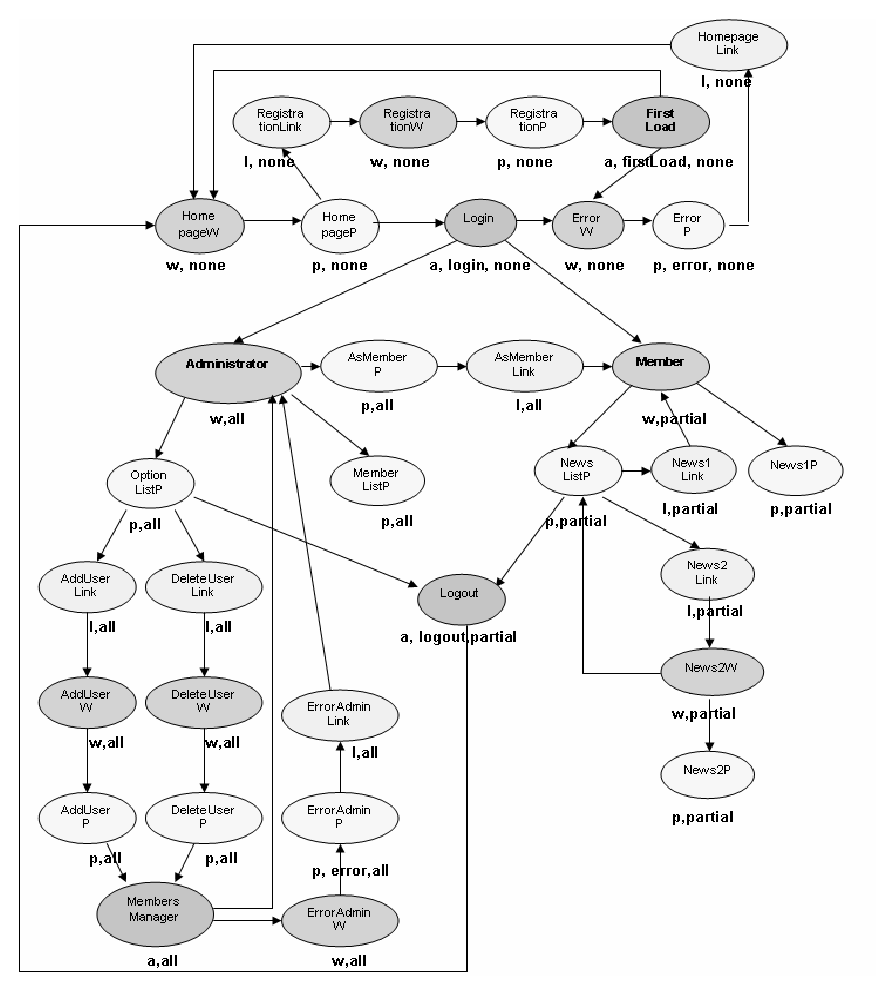
\includegraphics{figura4.eps}}}
\caption{WAG with access policies \label{fig4}}
\end{figure}

A direct consequence of such extensions is the elimination of ``private'' labels. In fact now we cannot only distinguish private pages and public pages accessible by anonymous users, but also we must distinguish private pages accessible by authorized users and private pages accessible by the administrator.

We think ``private'' label has became insufficient now, hence we introduce a new correctness axiom called ``accessibility''; it can assumes following values: 

\footnotesize
\begin{itemize}  
	\item	\textit{none} if web pages are visible by anonymous users;  
	\item	\textit{partial} if web pages are visible by authorized normal users;  
	\item	\textit{all} if web pages are visible by administrators.  
\end{itemize}

\normalsize
For the sake of simplicity, in our reference graph we consider only three users categories, but we are able to analyze models including more classes of users. They can be divided according to different levels of functionality or can be simply related to personal areas and resources (multiple subjects in the same category). Notice that possible extensions of the model does not compromise the validity of the reference example, whose correctness has been also proved in case of additional users categories.

In what follows we formalize and represent the graph grouping possible states of a user, independently by accessibility of pages s/he views at the moment. Hence we build a second supplementary model, for maintaining current states of users during navigation in WA: 

\footnotesize
\begin{itemize}  
	\item \textit{noLog} is an anonymous user which did not perform login operations;  
	\item \textit{member} is an authorized user which performed login as user of the WA;  
	\item \textit{admin} is an authorized user which performed login as administrator of the WA.  
\end{itemize}	

\normalsize
The state transitions permitted in this model can be represented by means of the simple following graph: 

\begin{figure}[ht]
\centerline{\scalebox{.35}{\includegraphics{figura5.eps}}}
\caption{User graph \label{fig5}}
\end{figure}

To verify some important specification, we synthesize following axioms:  

\footnotesize
\begin{itemize}
	\item a member cannot have administrator functions and an anonymous user cannot view pages belonging to a member:\\  
       $AG(member \Rightarrow !all );$     $AG(noLog \Rightarrow (!partial \wedge !all))$
	\item administrator can access to resources belongings to every authorized user:\\
       $AG( admin \Rightarrow (all \vee partial))$
\end{itemize}      

\normalsize
Besides, we previously introduced some \ctl specifications, that we now must correct according to new accessibility property, by removing specifications related to the ``private'' label. In particular about:

\footnotesize
\begin{itemize}
	\item initial state (Homepage):\\
			$A( none  \cup  login )$
	\item login and access to pages:\\ 
      $AG( login \Rightarrow  EF(partial \vee all) );$      $AG( logout \Rightarrow  A(none \cup  login))$
	\item error management:\\
			$AG (login \wedge EX EX error) \Rightarrow  A(none \cup  login )$
\end{itemize}

\normalsize
The above specifications point out that the accessibility logically replaces the correctness axiom related to private pages, providing a better precision in management of private resources of different users in the WA.

Now, verification process consists of establishing if state transitions in the model are coherent with accessibility of the pages. Hence, we define further NuSMV module besides \textit{MAIN} one; by means of it we synchronize user state transitions according to WA state transitions. For this purpose we use the ``stateName'' variable passed as input parameter every time the module is started. 


\section{From XMI to SMV}\label{xmi}
\subsection{Features of the tool}
Design documentation expresses the business logic of the WA in a visual fashion by using UML. Main benefit of UML is to allow representation of all the components of a WA by means of diagrams, notations and extension mechanisms. Conallen \cite{cona-02} defined new kinds of elements inside a metamodel and introduced a set of new stereotypes and new icons to represent components like static web pages as well as dynamic ones, frames, forms and to model interactions with databases.

To use UML diagrams in conjunction with Model Checking techniques for performing automatic verification, we implemented a component which is able to automatically translate a WA diagram, exported by an UML tool as XMI file, in the corresponding WAG; then, the WAG is translated in NuSMV code given as input to the model checker. Figure \ref{fig6} shows the location of this component, called \textit{XMI2SMV}, within the tool: 

\begin{figure}[ht]
\centerline{\scalebox{.4}{\includegraphics{figura6.eps}}}
\caption{XMI2SMV component within verification tool \label{fig6}}
\end{figure}

The \textit{XMI2SMV} component includes three packages, according to three principal features it has.

\textbf{XMIManager}. It imports UML diagram as XMI file, then it analyzes XMI file and extracts information about the FSM representing the WA.

More specifically, we reach this goal by means of realization of a \textit{State Table}; it stores relationships between the WA as web system and the same WA as FSM, where states and state transitions respect fundamental principles of the mathematical model.  

The class named ``StateTableCreator''is the main class of the package. It builds the \textit{State Table} by analyzing tags in the \textit{.xmi} document and filling two preliminary tables: \textit{Class Table}, which contains all the classes declared in the XMI file, and \textit{Transition Table}, which contains all declared associations in the XMI file. These two tables include information for building the \textit{State Table}; the ``StateTableCreator'' is able to rebuild the WAG according to XMI model by converting each class and every association in a state or in a state transition of the WAG.

\begin{figure}[ht]
\scalebox{.5}{\includegraphics{classe1.eps}}
\caption{StateTableCreator class \label{fig7}}
\end{figure}

A simple example will make clear the approach:

\footnotesize
\begin{itemize}
	\item every class targeted as ``Server Page'' will become a state labeled as ``action''; 
	\item every class targeted as ``Client Page'' will make both a state labeled as ``page'' and a state labeled as ``window''; 
	\item the declaration of the ``Frameset'' class will elicit elimination of some just created windows, because the corresponding pages are displayed in the same window;  
	\item every association link will become a state labeled as ``link''. 
\end{itemize}

\normalsize
Result is a basic and incomplete WAG: it has only nodes and arcs coming from the State Table. Correctness axioms will be assigned to the nodes by the following Graph Manager package.

\textbf{Graph Manager}. It is the main package of the tool, because it:

\footnotesize
\begin{itemize}
	\item calls main classes of connected packages to start operations like WAG creation or SMV code building;
	\item	manages the labeling of the states in the model according to correctness axioms;
	\item	internally stores WAG by means of suitable data structures, such as an \textit{adjacency matrix} and a \textit{vector of ``nodes''}.
\end{itemize}

\normalsize
More specifically, this package assigns the following labels to each node of the model (according to the fundamental correctness axioms described in previous sections): \textit{firstLoad}, \textit{login} and \textit{logout} which are about mechanisms of user authentication; \textit{error} which is about management of error pages; \textit{none}, \textit{partial} and \textit{all} which are about accessibility of private pages. 

However, to identify the states satisfying the above properties, the \textit{Graph Manager} needs information about main pages of WA. Hence WA designers have to provide a XML file, containing names of: homepage,	registration server page, both login and logout server pages, private pages displayed after either administrator or user login (and linked to logout page), error pages and so on. Each name is used by a function of ``Setting'' class; it selects the node of the graph corresponding to a specific web page and assigns to it the label related to the appropriate axiom of correctness.  

To inspect the graph or to select a specific node, the \textit{Graph Manager} exploits its internal model of the WAG. It is based on two special structures: an \textit{adjacency matrix}, where are stored --for each node-- information about connections with adjacent nodes, and a \textit{vector of ``Nodes''}, where each ``Node'' is a vector containing the name of the specific node followed by labels of the axioms of correctness.

Finally, when WAG is completed, ``addSpecification'' function allows to add \ctl specifications to the model; hence for each specification, ``WagManager'' class initializes a new class ``Specification'' and stores \ctl specifications in its \textit{formula} field.

%\begin{figure}[ht]
%\centerline{\scalebox{.5}{\includegraphics{classe2.eps}}}
%\caption{Graph and Node structures used in Graph Manager package \label{fig8}}
%\end{figure}

\textbf{SMVManager}. The third package of the tool builds the SMV code related to the WA, whose model and \ctl specifications are provided by the \textit{Graph Manager}. ``SMVGenerator'' is the main class of the package and coordinates following actions:

\footnotesize
\begin{itemize}
	\item	analysis of all the WAG states to obtain information useful for the translation of the model in the corresponding NuSMV formalism;
	\item	building and syntactic arrangement of \textit{MAIN} module contents modeling the WA states;
	\item	building and syntactic arrangement of the further \textit{SYNCHRO} module contents modeling the user state;
	\item	adding of the correctness axioms in the \textit{MAIN} module;
	\item	performing the SMV code automatic verification.
\end{itemize}

%\begin{figure}[ht]
%\centerline{\scalebox{.5}{\includegraphics{classe3.eps}}}
%\caption{SMVGenerator class \label{fig9}}
%\end{figure}

\normalsize
As previously stated, to perform such actions, the package is equipped with a XML file, containing information to be inserted in SMV code and related to every WAG. 

\section{Related Work}\label{related}
Tin this Section we briefly describe the more relevant proposals in the field of web application verification.
Some approaches consider the web similar to a database, hence propose conceptual models of its structure; more recent approaches focus on web applications under a web engineering point of view. A complete review of all the modeling techniques is in \cite{fraternali-99}.

HDM \cite{gar-pao-93} is one of the first model-driven design of hypermedia applications; successive proposals are RMM\cite{isa-sto-95}, Strudel \cite{fer-98} and Araneus\cite{atz-mec-mer-98}. They all build on the HDM model and support specific navigation constructs. In particular, Araneus describes the data structure based on the entity relationship model.  

In the second perspective, that is considering a Web Application as a software object, several modeling techniques have been adopted. Conallen \cite{cona-02} proposes a UML-based methodology. The main benefit of the method is the feature which allows to represent all the components of a Web Application using a standard UML notation. OOHDM \cite{ros-sch-02} is an object-oriented method to represent design structure in WAs. The method considers Web Applications as navigational views over an object model and provides some basic constructs for designing the navigation model. UWE \cite{koch-kraus-02} is an object-oriented, iterative and incremental approach based on the UML. 
 
WebML \cite{cer-fra-mat-02} introduces graphical and XML representation of concepts for designing Web Applications. Anyway, all the proposals are modeling techniques. To perform verification of a WA it is necessary to use verification or testing techniques. 

The method proposed in \cite{ric-ton-02} is based on a UML model of WAs and considers the testing and validation of the developed web system. In \cite{antoniol}, a Web Application analysis based on queue models is proposed. Finally, in \cite{dilucca} the authors verify the correct use of duplicated pages inside a web constructed using HTML language and ASP code. Once again the proposed method does not consider a formal approach.

On the other hand, model checking based on a $\mu-calculus$ language has been used in \cite{de-alfaro-01}, but the approach does not present the analysis of dynamic pages. Anyway in this work the author considers a model of the web like a graph in which states are pages and transitions between states are hyperlinks in the pages. Hence hyperlinks cannot be qualified by properties as we do.

In \cite{stotts-98} the automata are used to outline the framework of the links in a hypertext. Hence a branching temporal logic (HyperText Logic) HTL is defined. By means of it a sequence of transitions between states in the automata can be described. The logic is also used to verify the propositions of the temporal logic, but again dynamic pages are not considered.

In \cite{veriweb} a tool for automatically discovering and systematically exploring web-site execution paths is proposed: it is a spider-like program which follows all the possible static links in every HTML web page and surfs through all dynamic components of a web application, including both submission/execution forms and client-side scripts. During web site examination, the tool allows to check for many kind of errors, in single web pages as well as in a navigation paths, by means of a regression test. However, the WA must be already implemented in HTML to perform all tests. Hence possible discovered errors have a great cost of repairing.

\section{Conclusion}
In this paper, we proposed a formal model and a tool for verification of the UML design of WA. The method is based on model checking and the properties to be verified on the model are expressed in \ctl. The implemented system parses the XMI code obtained as output of a UML design tool and builds the \smv model where properties are verified.

The proposed method and tool have the main advantage of joining the two phases of design and verification of a WA in a single automated activity. Hence, we can say \textit{WAVer} performs an ``a priori'' verification of the WA design, saving time and costs and increasing software quality; the verification is fully automated because \textit{WAVer} embeds NuSMV model checker which establish system correctness. Simulation and results prove the benefit of our approach.

\bibliographystyle{plain}
\bibliography{long,model}

\end{document}